\section{Methods - Network pipeline} \label{s:N_I:methods}

The network pipeline can be broken in several stages 1) the graph is constructed from RNA-seq data and community detection algorithm is applied; 2) compute the most important genes in each community; 3) find the representation of the selected genes to the samples; 4) apply clustering analysis to find the disease subgroups; summarised in \cref{fig:N_I:network_pipeline}.

It is worth noting that the \acrfull{pgcna} developed by \citet{Care2019-ij} is adapted for the aims of this project. The authors created PGCNA to integrate multiple gene expression dates whereas the method developed in this project uses a single gene expression dataset (to create the network) into which other data types (i.e., mutations and TF) are integrated. The following sub-sections are covering each step in the network pipelines and how were adapted for the project requirements.

\begin{sidewaysfigure}
    \centering
    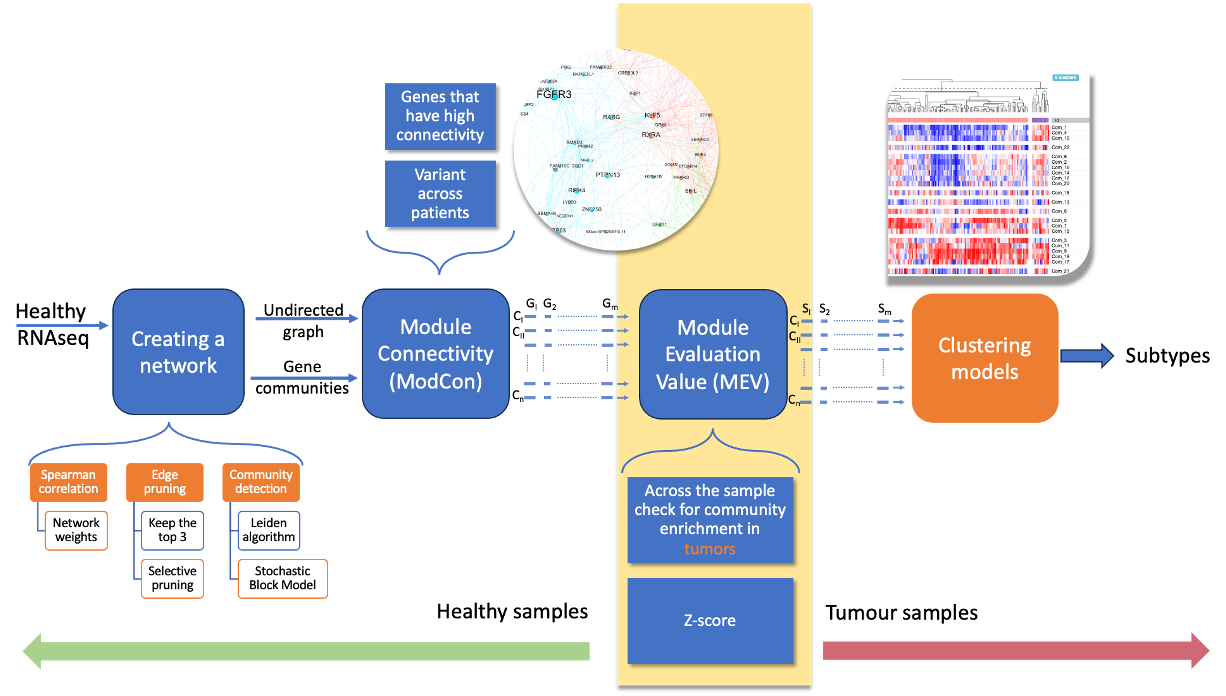
\includegraphics[width=1.0\textwidth,keepaspectratio]{Sections/Network_I/Resources/Methods/network_pipeline.png}
    \caption[The integrative network pipeline]{Network pipeline developed to integrate mutation burden, transcription factors (TF), and the non-tumour dataset; supporting the methods described in \cref{s:N_I:methods}. The first step is to build the network, which includes: 1) computing the edge weights with Spearman correlation and applying modifiers to integrate mutation data; 2) selective edge pruning, where TF are allowed a higher minimum degree; 3) applying community detection algorithms such as Leiden or Stochastic Block Model. The second step involves extracting the top 100 most well-connected nodes in a community using the ModCon score. The Module Evaluation Value (MEV) is then computed to assess the enrichment of the selected genes from each community in the MIBC samples from TCGA. Finally, the MEVs are grouped together using cluster analysis methods.}
    \hfill
    \label{fig:N_I:network_pipeline}
\end{sidewaysfigure}

%% Gene filtering will be with Network Construction
\subsection{Gene filtering} \label{s:N_I:gene_filtering}

The genes are filtered by the same aggressive approach as in the cluster analysis chapter, \cref{s:cs:methods}, selecting the top on 4000 genes, for tumour networks (\cref{s:N_I:tum}), and 5000 for P0 networks (\cref{s:p0}). These are the genes with the highest median/standard deviation and are expressed in at least 90\% of the samples. A Spearman Correlation matrix is then built, where the correlation of two genes represents the edge weights while network nodes are the genes themselves. 

% There is not specific rationale for choosing 3K or 5K top most varied genes. 
For cluster analysis usually a third of the expressed genes (3000-4000 genes) are used (e.g. TCGA subtyping - \citet{Robertson2017-mg}). When selecting only the top 3K, there are few genes included that are commonly mutated in the tumour dataset, so the threshold was lowered to 5K.

\subsection{Weight modifiers} \label{s:N_I:weight_modifiers}

The network weights are modified to integrated the mutation burden across TCGA cohort into the network. The changes are applied after the Spearman correlation matrix is computed and before the selective edge pruning. Thus, the integration of the mutation burden influences the number of connections a gene has. This is important for the Module Connectivity score which ranks genes by their importance in the community considering the node's edges and their weights; the score is later introduced in \cref{s:N_I:methods_modcon}.

% What is the desired behaviour
There are two mutation integration strategies proposed, one that rewards or promotes the mutated genes in the network by increasing the edges weights (i.e. correlation values). The other is the reverse and penalising the mutated genes by reducing their weights in the graph. The desired behaviour is for the highly mutated genes such as \textit{TP53} or \textit{TTN} (both are mutated in $\sim$50\% of the MIBC cohort) to have the largest change by either doubling their weights or reducing to almost 0. Concurrently, the non-mutated genes should not be effected by the weight modifiers.

\begin{equation} \label{eq:w}
    \large{
    w(x) = \log_2(x+1)
    }
\end{equation}

\begin{equation} \label{eq:weight_modifiers_1}
    \large{
    \text{f}(w) = 
    \begin{cases} 
    \frac{\max(w) + w}{\max(w)} & \text{if reward modifier}, \\
    \frac{\max(w) - w}{\max(w)} & \text{if penalised modifier}.
    \end{cases}
    }
\end{equation}

% Introduce the equation
To achieve the desired behaviour the \cref{eq:weight_modifiers_1} is used where where $w$ is the $log_2$ transformed of the mutation burden shifted by 1 (to avoid undefined values at 0 see \cref{eq:w}, $x$ represents the mutation burden taken from TCGA dataset.  The arc-like behaviour of the function is shown by the red line in \cref{fig:N_I:modifiers}. Most of the mutated genes increase the weights value up to $50\%$ (value of $1.5$) for reward while the opposite is true for the penalised modifier. 

% \begin{equation} \label{eq:norm3_func}
% \text{f}(w) = \frac{\max(w) + w}{\max(w)}
% \end{equation}

% \begin{equation} \label{eq:pen_func}
% \text{f}(w) = \frac{\max(w) - w}{\max(w)}
% \end{equation}

\begin{figure}[!htb]    
    \centering
    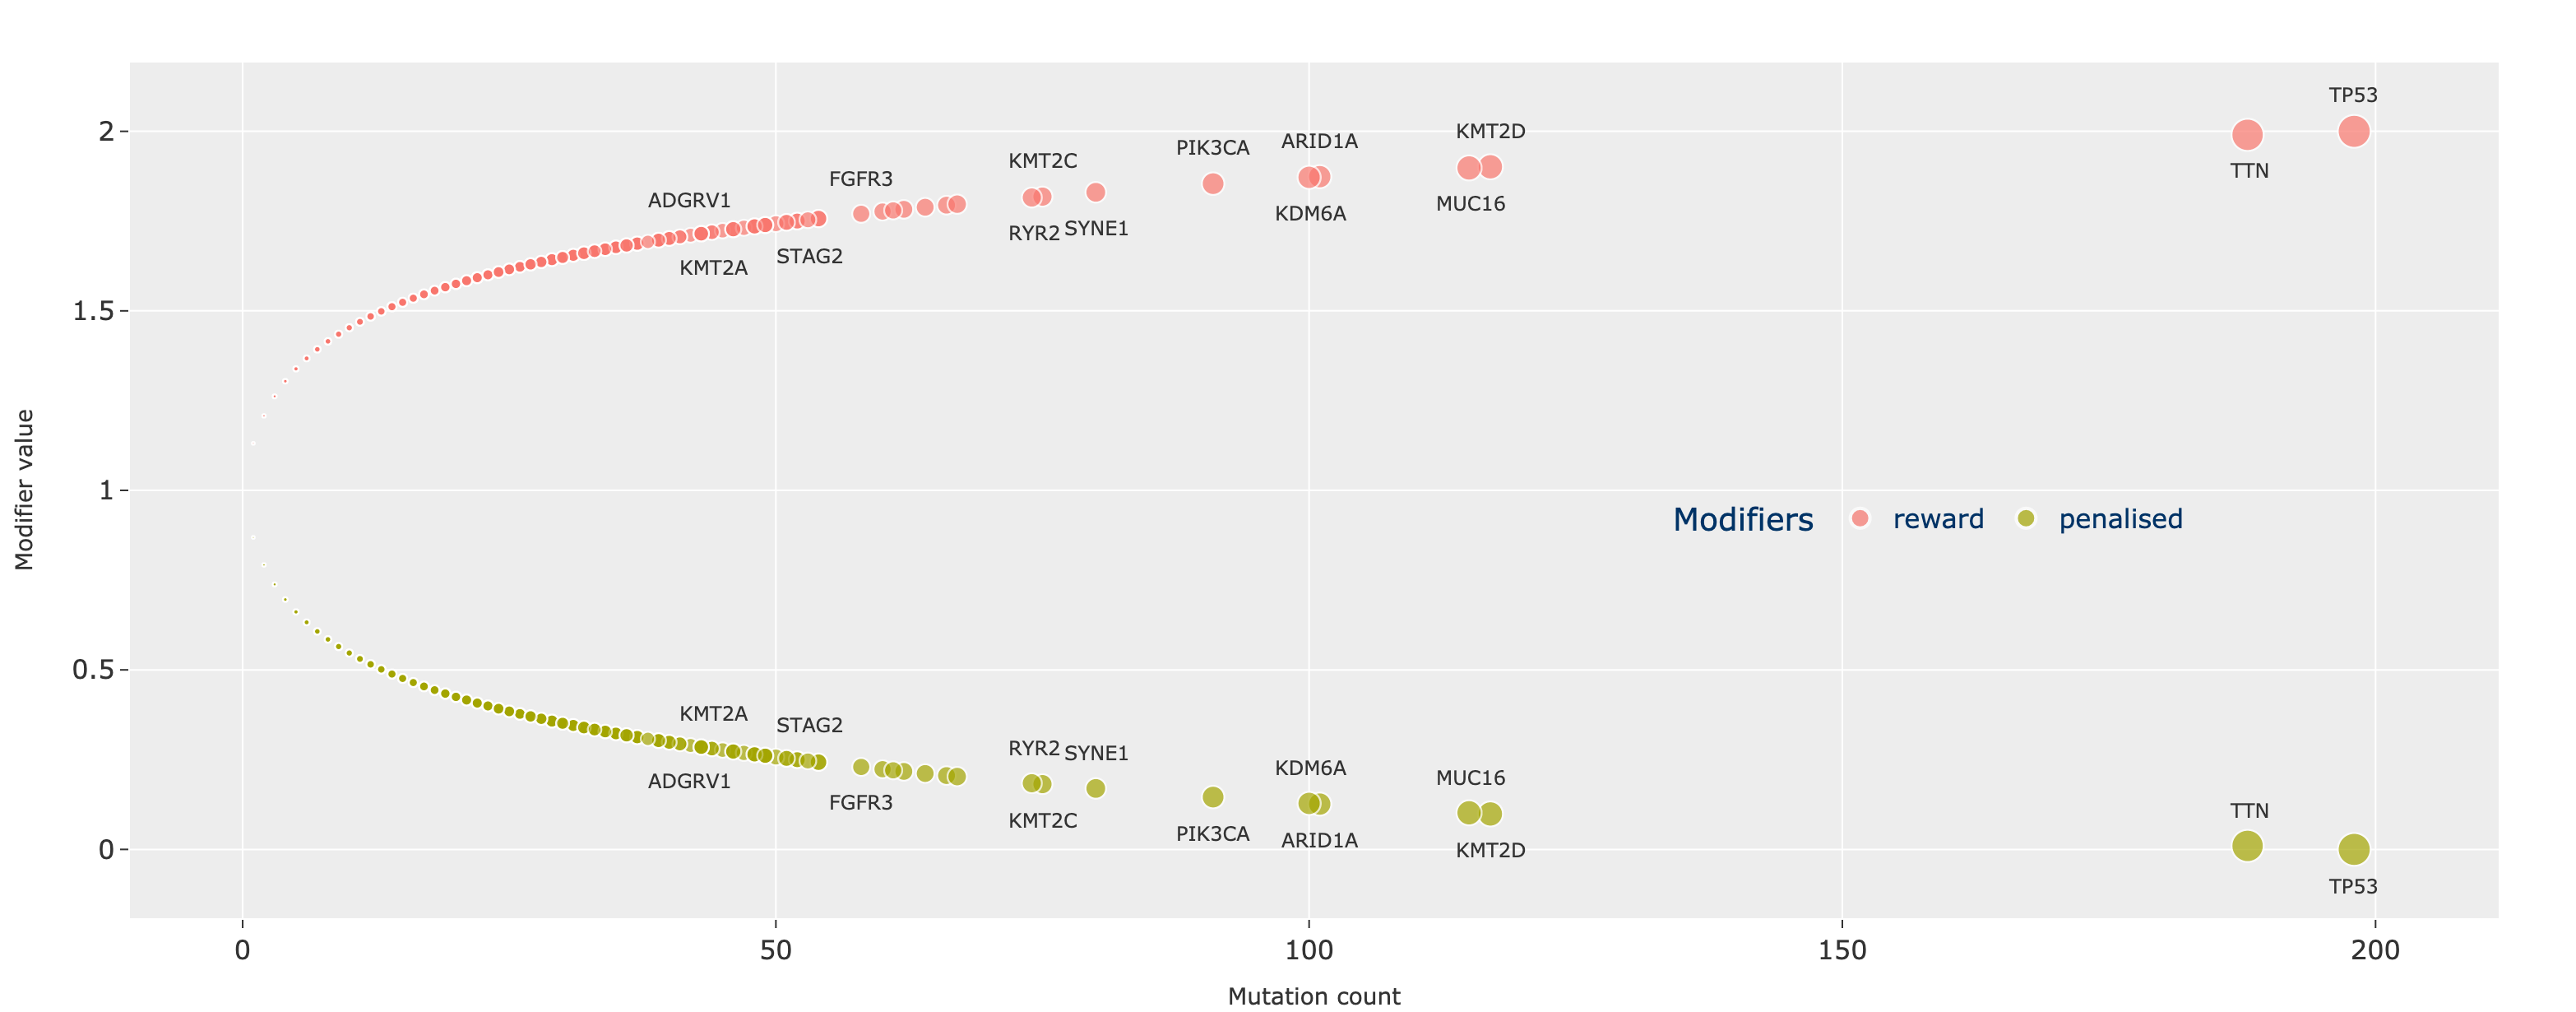
\includegraphics[width=1.0\textwidth,keepaspectratio]{Sections/Network_I/Resources/Methods/modifiers.png}
    \caption[Reward v1 vs Penalised edge weight modifiers]{Representing the two weight modifier strategies employed at the network construction stage. The red, reward strategy, awards the genes that have a high burden across the cohort. Conversely, the  penalised strategy decreases the edges' strength for highly mutated genes. In both cases, the non-mutated genes remain unchanged.}
    \label{fig:N_I:modifiers}
\end{figure}

% Selective edge pruning
\subsection{Selective edge pruning} \label{s:N_I:methods_edge_pruning}

% Why there is a need for edge pruning
For a network of 5000 nodes there are $1.24\text{x}10^6$ possible edges, retaining all of them makes the network challenging to analyse and as the following section will show it influences the community detection methods. In \citet{Care2019-ij}, the authors explore different edge pruning strategies and found that on their datasets (Glioblastoma and Breast cancers), an aggressive strategy yields the best result by their score (SCES), which considered network metrics and Gene Ontology results. The strategy keeps the 3 top most correlated genes, meaning that the pruning occurs once for each node at the source node, resulting in a minimum degree of 3. It is worth pointing out that highly correlated destination nodes can have degree much larger than 3\footnote{For example, gene A is in the top 3 of gene E, and the reverse is not valid, then A will have a degree of 4 or the node has edges to the other four different genes; given that gene E is not in the top correlation of gene A}. 

% Default values
The authors from PGCNA build networks with 3-10 minimum edges for nodes and observed that using the Modularity score\footnote{Modularity maximisation is covered in more detail in \cref{s:lit:mod_max}.} and the number of communities, the graphs where nodes have a minimum 3 degree yields the best results. In addition to the two criteria network, the \citet{Care2019-ij} assess their performance over the biological findings using SCES.

The edge pruning approach from \citet{Care2019-ij} was adapted to prioritise a list of genes from Human Transcription Factors \citep{Lambert2018-el}. The \acrlong{tf} are genes with a higher impact on the other genes by regulating their expression. Therefore, the selective edge pruning strategy would allow the TF to have a higher number of edges than the standard genes. This chapter explores how the selective edge pruning influences the networks, the Leiden algorithm and the MIBC subgroups, while the next chapter, \cref{s:N_I:sel_pruning}, finds the appropriate number of connections for \acrshort{tf}.

% Community detection
\subsection{Community detection} \label{s:N_I:methods_comm_detection}


Once the network is built, a community detection algorithm is applied to find the sub-networks of genes. The purpose is to identify genes that are correlated with each other, which may resemble some parts of the biological process. In this project two main classes of community detection algorithms are explored: Leiden and Stochastic Block Model (SBM). The first algorithm is a popular method used to find partitions, blocks (=communities,,modules) used in the work of \citet{Care2019-ij}. However, as it was introduced in depth in the background chapter, \cref{s:lit:comm_detect}, Leiden may find non-existent structure in the data \citep{Peixoto2021-jx} whereas SBM addresses this issue by employing a Bayesian approach \citep{Peixoto2019-fg}. 

The project uses both methods, initially, Leiden with Modularity Score in the tumour and P0 derived networks in \cref{s:N_I:tum,s:p0} in this chapter. The next results chapter \cref{s:N_I} compares the Leiden algorithm with SBM, and the last one, \cref{s:N_II}, only uses the Stochastic Block Model.


% Finding the relevant genes
\subsection{Important genes in communities} \label{s:N_I:methods_modcon}

In the work of \citet{Care2019-ij}, the Module Connectivity (ModCon) score is computed for each gene to identify important nodes within each community, weighted by the gene expression values across the dataset(s) used. The research in this project does not integrate multiple gene expression datasets, resulting in a simplified version of some initial variables involved in the ModCon computation.

% Connectivity and perncetile expression
The connectivity ($conn$) of a node is computed according to \cref{eq:connectivity}, which represents the sum of the weights ($w$) of the edges between nodes $i$ and $j$ within the same community, $C$. The equation quantifies the total strength of the connections a node has within its community. It is worth noting that when a weight modifier is applied to integrate the mutation burden, the connectivity variable reflects those changes.

\begin{equation} \label{eq:connectivity}
    conn = \sum_{\substack{i, j \in C}} w_{ij} \\
\end{equation}

% Percentile expression
The variable $perExp$ represents the median percentile expression of a gene across the samples $PR(X)$; see \cref{eq:percent_exp}. The percentile expression is calculated as the normalised rank of gene $i$ (\(X_i\)), as defined in \cref{eq:exp_rank}. This variable ensures that the ModCon score is weighted by considering the relative expression level of a gene within the dataset, in comparison to other genes.

\begin{equation} \label{eq:percent_exp}
    perExp = \text{median}\left(\text{PR}(X)\right)
\end{equation}

\begin{equation} \label{eq:exp_rank}
    \text{PR}(X_i) = \frac{\text{rank}(X_i)}{n} \times 100
\end{equation}

% Var within
In the work of \citet{Care2019-ij}, varWithin ($med$) is described as the median quantile coefficient of dispersion across all datasets. Since this project uses only a single dataset to construct the network, the variable simplifies to the median expression, as shown in \cref{eq:varWithin}.


\begin{equation} \label{eq:varWithin}
    med = \text{median}(X) \\
\end{equation}

% Dispersion (varAcross)
The varAcross variable, denoted as $disp$, is defined as the Quartile Coefficient of Dispersion (QCD) of the percentile expression within the dataset, following \citet{Care2019-ij}. This measure of dispersion quantifies the variability of the percentile expression and is less sensitive to outliers than other measures of variance. Although \citet{Care2019-ij} originally applied this measure across multiple datasets, in this project, it is applied within a single dataset, without taking the median; the variable is defined in \cref{eq:varAcross}. Lower values of $disp$ indicates that the variable has similar values across the datasets


\begin{equation} \label{eq:varAcross}
    disp = \frac{Q3 - Q1}{Q3 + Q1}
\end{equation}

Combining all the terms, the ModCon score is defined as shown in \cref{eq:modcon}. This score reflects the importance of a gene within its community by considering several factors: the connectivity ($conn$), which measures the extent of the gene's interactions within the community; the median expression ($med$), representing the overall expression level of the gene; the percentile expression ($perExp$), which indicates the gene's expression relative to other genes in the dataset; and the dispersion ($disp$), which accounts for the variability in the gene's expression. In this context, lower dispersion increases the score, while higher dispersion reduces it, as the term $(100 - disp)/100$ decreases with increasing dispersion. The final score is a product of these factors, where higher connectivity, higher expression levels, and greater consistency in expression (lower dispersion) all contribute positively to the ModCon score.

\begin{equation} \label{eq:modcon}
    ModCon = conn^2 \cdot perExp \cdot med \cdot \frac{100 - disp}{100}
\end{equation}

% Representation of genes across samples & Clustering
\subsection{Bridging the gap to samples} \label{s:N_I:mev}

After the genes are ranked with ModCon the top 100 genes are selected as representative. The top 25 genes are selected in PGCNA \citep{Care2019-ij} using the same dataset for both building the network and the disease subtyping. However, when the non-tumour graphs are computed, there are situations when the most varied genes in the non-cancerous dataset are not present in the tumour dataset. To account for this, more genes, 100, are then selected from each community. These chosen genes are used to compute the Module Evaluation (MEV) score \citep{Care2019-ij} to find the gene's representation across samples. The MEV is described in the pseudo-code in \cref{alg:N_I:mev}.

\begin{algorithm}
\caption{Module Evaluation Value }\label{alg:N_I:mev}
    \begin{algorithmic}
    \For{each community in all the network communities}     
        \For{each gene in the top 100 genes} 
            \State $z\_score=$ for the quantile normalised $log2$(gene expression)
            \For{each patient in all samples}  
                \State $MEV=$ sum of the \textit{z-score}  \Comment{Only for the top selected genes}
            \EndFor
        \EndFor
    \EndFor
    \end{algorithmic}
\end{algorithm}

The output of the \cref{alg:N_I:mev} is a $M\text{x}N$ matrix, with $M$ communities and $N$ samples in the targeted dataset. On this matrix cluster analysis can then be applied to find the cancer subtypes. Thus, the methods and analysis tools developed in the previous chapter on cluster analysis, \cref{s:clustering_analysis}, can be applied to find the appropriate cluster configuration (see \cref{s:ap:P0_cs_analysis}).


\subsection{Implementation details} \label{s:N_I:implementation}

The experiments performed in this section are using a modified version of the PGCNA Python packaged developed by \citet{Care2019-ij}. It is worth noting that PGCNA was developed to support gene expression integration at the network level i.e., use the median expression across the given datasets. For the needs of the project this was not needed and a single gene expression is used to created the networks but with the new data integration. The adapted version is published along with the software in this project see \cref{s:ap:software} from Appendix.

% Changes made
Initially the correlation values between genes is changed based on the weight modifiers proposed in \cref{fig:N_I:modifiers} and their effect are explored in both tumour and P0 networks in \cref{s:N_I:tum,s:p0}. Then, the number of edges is selectively altered for a given subset of genes, the experiments are covered in \cref{s:N_I:sel_pruning}. 





